\documentclass{beamer}



\usepackage{listings}
\usepackage[english]{babel}
\usepackage{amsmath}
\usepackage[latin1]{inputenc}
\usepackage{units}
\usepackage{colortbl}
\usepackage{multimedia}
\usepackage{bm}
\usepackage{subcaption}
\usepackage{algorithm2e}
\usepackage{algorithmic}

% Math commands
\newcommand{\sys}{S}
\newcommand{\diss}{d}
\newcommand{\learn}{\mathcal{A}}
\newcommand{\free}{\mathcal{M}}
\newcommand{\D}{\mathcal{D}}
\newcommand{\R}{\mathbb{R}}
\newcommand{\nsamp}{N}
\newcommand{\norm}[1]{\left\lVert#1\right\rVert}

\newcommand{\E}{\mathbb{E}}
\newcommand{\mdl}{M}
\newcommand{\mdlstruc}{\mathcal{M}}

% Colors
\definecolor{darkgreen}{RGB}{20,150,50}
\definecolor{Periwinkle}{rgb}{0.0, 0.0, 0.0}
\definecolor{darkgreen}{RGB}{20,150,50}
\definecolor{orange}{RGB}{204, 85, 0}

\mode<presentation>
{
  \usetheme{Boadilla}
  \useoutertheme{infolines}
  \setbeamercovered{transparent}
}


\title[In-context learning sysid]{\textsc{In-context learning for model-free system identification}}


%\author[]{Marco Forgione\inst{1}, Filippo Pura\inst{1}, Dario Piga\inst{1}}
\author[]{Marco Forgione, Filippo Pura, Dario Piga}

\institute[IDSIA]{
	\inst{}IDSIA Dalle Molle Institute for Artificial Intelligence SUPSI-USI, Lugano, Switzerland
	}


\date[]{September 7, 2023}
%\date[]{\today}


\subject{System Identification, Meta Learning, In-context Learning, Transformers}

\newcommand{\book}{\includegraphics[width=10pt]{fig/proceeding-logo.jpg}}
\newcommand{\github}{\includegraphics[width=10pt]{fig/github-logo.jpg}}


\begin{document}

\begin{frame}
  \titlepage
\end{frame}



\begin{frame}{Standard system identification/supervised machine learning}
%Standard system identification workflow:
\begin{enumerate}
\item Collect dataset $\D = (u_{1:N}, y_{1:N})$ of input/outputs
%$$\D = u_{1:N}, y_{1:N}$$
from  system $\sys$.
\item Apply an algorithm to estimate a model $M(\hat \theta)$ of $\sys$:
$$\hat \theta = \learn(\D)  \qquad \text{e.g.  }  \learn(\D)  = \arg \min_{\theta \in \Theta} \mathcal{L}(\D, M(\theta))$$
\item Make predictions/simulations using the model on new data:
%$$\hat y_k = M(u_{1:k-1}; \theta^*)$$
$$\hat y^*_{1:M} = M(u^*_{1:M}; \hat \theta)$$
\end{enumerate}
\pause
Researchers keep on improving learning algorithms and model structures.\\
Can we automate this process?
Can we \structure{learn the learning algorithm} itself?\\
\pause

\vskip .5em
\structure{Meta learning} tries to answer this question.


 	\begin{itemize}
	\item[\book]
		\begin{tiny}
	\structure{J. Schmidhuber.}
     Evolutionary principles in self-referential learning, or on learning how to learn. \vskip -1em
     \emph{Diploma Thesis, TU Munich, 1987}
		\end{tiny}\\

	\item[\book]
		\begin{tiny}
	\structure{T. Hospedales et al.} % A. Antoniou, P. Micaelli, and A. Strokey
     Meta-Learning in Neural Networks: A Survey.
     \emph{IEEE Transactions on Pattern Analysis and Machine \vskip -1em
      Intelligence, 2022}
		\end{tiny}\\

    \end{itemize}

\end{frame}


\begin{frame}{Our meta learning setting}
\begin{itemize}
%Meta learning setting
 \item We have an \structure{infinite stream} of datasets from a distribution $p(\D)$:
  $$\{\D^{(i)} = (u_{1:\nsamp}^{(i)}, y_{1:\nsamp}^{(i)}), \,\, i=1,2,\dots, \infty \}$$
 \item $\D^{(i)}$ generated by \structure{random system} $\sys^{(i)}$ and input realization $u_{1:\nsamp}^{(i)}$
 \item Different but \structure{related to each other}. There's a learnable structure!
\end{itemize}
\vskip 1em
\pause
Can we get better at identifying $\sys^{(i)}$ as we observe more datasets $\D^{(j)}$?
\pause
\vskip 1em
\begin{itemize}
\item $p(\D)$ may be a \structure{physical simulator} where we can change settings
\item The learned algorithm could then be applied to \structure{real data}
% with insight
\end{itemize}
\vskip 1em
\pause
Meta learning from a \structure{finite collection} would also be interesting...
\end{frame}

\begin{frame}{In-context learning}
Many meta learning strategies around. Here focus on \structure{in-context learning}.
\vskip 1em
\begin{itemize}
\item \structure{Transformers} are expressive  as \structure{a programming language}%are sufficiently expressive to \structure{represent algorithms}.
\item We make Transformers \structure{behave like algorithms}. We provide:
\begin{itemize}
\item A \structure{context}, namely an input/output sequence of a system
\item A \structure{task}, like predicting the next output or simulating for more steps
\end{itemize}
\item The Transformer must \structure{learn to identify} the system to solve the task!
\end{itemize}
\vskip 1em
%\pause
Context + task may be seen as a \structure{prompt} to a Large Language Model, which can then
\structure{continue the word sequence} in an optimal way.

\vskip 2em

\begin{itemize}
	\item[\book]
		\begin{tiny}
	\structure{G.~Weiss et al.} % A. Antoniou, P. Micaelli, and A. Strokey
     Thinking like Transformers.
     \emph{38th International Conference on Machine Learning (ICML 2022).}
		\end{tiny}
		
	\item[\book]
		\begin{tiny}
	\structure{S. Garg et al.} % A. Antoniou, P. Micaelli, and A. Strokey
     What Can Transformers Learn In-Context? A Case Study of Simple Function Classes.
     \emph{36th Conference on \vskip -1em Neural Information Processing Systems (NeurIPS 2022).}
		\end{tiny}

	\item[\book]
		\begin{tiny}
	\structure{T. Brown et al.} % A. Antoniou, P. Micaelli, and A. Strokey
     Language Models are Few-Shot Learners.
     \emph{34th Conference on  Neural Information Processing Systems \vskip -1em (NeurIPS 2020).}
		\end{tiny}\\

\end{itemize}
\end{frame}

\begin{frame}{Two system identification problems}
\begin{columns}[t]
\column{.48\textwidth}
\begin{block}{One-step prediction:}
$$\hat y_{k+1} = \free_\phi(u_{1:k}, y_{1:k})$$
\begin{itemize}
\item $(u_1, y_1) \rightarrow \hat y_2$
\item $(u_{1:2}, y_{1:2}) \rightarrow \hat y_3$
\item $(u_{1:3}, y_{1:3}) \rightarrow \hat y_4$
\item $\dots$
\item $(u_{1:\nsamp-1}, y_{1:\nsamp-1}) \rightarrow \hat y_\nsamp$
\end{itemize}
\end{block}
\column{.48\textwidth}
\begin{block}{Multi-step simulation}
\vskip -1em
$$\hat y_{m+1:N} = \free_\phi(u_{1:m}, y_{1:m}, u_{m+1:N})$$
%\vskip .8em
Meta-model receives:
\begin{enumerate}
\item Full input/output $(u_{1:m}, y_{1:m})$
\item Input-only trajectory $u_{m+1:\nsamp}$
\end{enumerate}
%\vskip 1em
and generates simulation:
$\hat y_{m+1:N}$
\vskip 1em
\begin{itemize}
\item $u_{1:m}, y_{1:m}, u_{m+1:N} \rightarrow \hat y_{m+1:N}$
\end{itemize}
\end{block}
\end{columns}
\pause
\vskip 1em
\begin{itemize}
\item If we manage to train a Transformer $\free_\phi$  to solve such problems \structure{for a class of systems}, it becomes a \structure{meta model} of that class!
\item $ \free_\phi$ becomes \structure{as powerful as a system identification algorithm}!
\end{itemize}
\end{frame}

\begin{frame}{Meta model training}
\begin{columns}[t]
\column{.48\textwidth}
\begin{block}{One-step prediction:}
\begin{tiny}
$$\hat \phi = \arg \min_\phi \mathcal{L}_{\rm pred}(\phi)$$
\begin{equation*}
	\label{eq:one_step_objective}
     \mathcal{L}_{\rm pred}(\phi) = \E_{p(\D)}
    \left [ \sum_{k=1}^{\nsamp-1}
    \norm{y_{k+1} -
    \free_\phi (y_{1:k}, u_{1:k})
    }^2
    \right ]
\end{equation*}
\vskip -1.5em
\begin{equation*}\label{eq:eq:one_step_objective_samples}
\mathcal{L}_{\rm pred}(\phi)  \approx  \frac{1}{b}
    \sum_{i=1}^b
    \sum_{k=1}^{\nsamp-1}
    \norm{y_{k+1}^{(i)} -
    \free_\phi (y^{(i)}_{1:k}, u_{1:k}^{(i)})}^2
\end{equation*}
\end{tiny}
\end{block}
\column{.48\textwidth}
\begin{block}{Multi-step simulation}
\begin{tiny}
$$\hat \phi = \arg \min_\phi \mathcal{L}_{\rm sim}(\phi)$$
\begin{equation*}
	\label{eq:simulation_objective}
   \mathcal{L}_{\rm sim}(\phi)  \! = \!  \E_{p(\D)}
    \left [
    \norm{y_{m+1:\nsamp} \! - \! \free_\phi (u_{1:m}, y_{1:m}, u_{m+1:\nsamp})
    }^2
    \right ]
\end{equation*}

\begin{align*}
	\label{eq:simulation_objective_samples}
     \mathcal{L}_{\rm sim}(\phi)   \approx
    \frac{1}{b}
    \sum_{i=1}^b
    %
    \norm{y_{m+1:\nsamp}^{(i)} - \free_\phi (u_{1:m}^{(i)}, y_{1:m}^{(i)}, u_{m+1:\nsamp}^{(i)})}^2
\end{align*}
\end{tiny}
\end{block}
\end{columns}
\pause
\vskip 1em
\begin{itemize}
\item Formally, just two \structure{boring supervised learning} problems.
\item The use of powerful architectures and \structure{training on a whole class} of dynamical systems
makes the outcome special.
\item If the optimization works out well, the Transformer becomes   a \structure{meta model} of the systems in $p(\D)$!
\item We have \structure{learned a learning algorithm!}
%The trained Transformer becomes \structure{as powerful as a learning algorithm}!
\end{itemize}
\end{frame}



%\begin{frame}{Transformer architectures}
%\begin{columns}[t]
%\column{.33\textwidth}
%\begin{center}
%One-step prediction:
%decoder-only ($\sim$ GPT-2)
%\begin{figure}
%\includegraphics[height=110 pt]{fig/architecture/decoder_architecture.pdf}
%\end{figure}
%\vskip 1em
%
%\end{center}
%\column{.69\textwidth}
%\begin{center}
%Multi-step simulation:\\
%encoder-decoder ($\sim$ language translation)
%\begin{figure}
%\includegraphics[height=130 pt]{fig/architecture/encoder_decoder_architecture.pdf}
%\end{figure}
%\vskip -.8em
%
%\end{center}
%\end{columns}
%\pause
%\vskip 1em
%\begin{itemize}
%	\item[\book]
%		\begin{tiny}
%	\structure{A. Vaswani et al.} % A. Antoniou, P. Micaelli, and A. Strokey
%     Attention is all you need.
%     \emph{30th Conference on  Neural Information Processing Systems (NeurIPS 2017).}
%		\end{tiny}\\
%\end{itemize}
%NLP architectures modified to process \structure{real-valued input/output sequences}.
%
%\end{frame}

\begin{frame}{Transformer architectures}
\begin{columns}[t]
\column{.33\textwidth}
\begin{block}{One-step prediction:}
\begin{figure}
\vskip 1em
\includegraphics[height=110 pt]{fig/architecture/decoder_architecture.pdf}
\vskip .8em
decoder-only ($\sim$ GPT-2)
\end{figure}
\end{block}
\column{.65\textwidth}
\begin{block}{Multi-step simulation}
\begin{figure}
\includegraphics[height=130 pt]{fig/architecture/encoder_decoder_architecture.pdf}
encoder-decoder ($\sim$ language translation)
\end{figure}
\end{block}
\end{columns}
\vskip 1em
%\begin{itemize}
%	\item[\book]
%		\begin{tiny}
%	\structure{A. Vaswani et al.} % A. Antoniou, P. Micaelli, and A. Strokey
%     Attention is all you need.
%     \emph{30th Conference on  Neural Information Processing Systems (NeurIPS 2017).}
%		\end{tiny}\\
%\end{itemize}
NLP architectures modified to process \structure{real-valued input/output sequences}.
\end{frame}


\begin{frame}{Experiments - System classes}
One-step prediction and multi-step simulation on two system classes:
%\vskip 1em
\begin{columns}[t]

\column{.48\textwidth}
\begin{block}{Linear Time Invariant (LTI):}
In state-space form, order $\leq 10$
\begin{align*}
x_{k+1} &= Ax_k + Bu_k\\
y_{k+1} &= Cx_k
\end{align*}
\vskip -.5em
\begin{itemize}
\item Random system matrices
\item $A$ constrained to be stable
\end{itemize}
\end{block}
\column{.48\textwidth}
\begin{block}{Wiener-Hammerstein (WH):}
\vskip .8em
\begin{figure}
\includegraphics[width=.7\textwidth]{fig/wiener_hammerstein.pdf}
\end{figure}
\begin{itemize}
\item Sequential LTI $\rightarrow$ $F(\cdot)$ $\rightarrow$ LTI
\item Random LTI, order $\leq 5$
\item $F(\cdot)$: random feedforward NN.
\end{itemize}
\end{block}
\end{columns}
\vskip 1em
\begin{itemize}
\item For both classes, input $u_{1:\nsamp}$ is a white Gaussian noise sequence.
\item This defines a $p(\D)$. We can generate infinite datasets!
\item Each dataset from a different input/system realization!
\end{itemize}

 	\begin{itemize}
	\item[\github]
		\begin{tiny}
		\url{https://github.com/forgi86/sysid-transformers}
		\end{tiny}\\
 \end{itemize}
\end{frame}

\begin{frame}{Experiments - one-step prediction results}
\begin{columns}[t]
\column{.5\textwidth}
\begin{center}
\begin{figure}
LTI: one sequence
\includegraphics[width=\textwidth]{fig/lin_one_step_single.pdf}
WH: one sequence
\includegraphics[width=\textwidth]{fig/wh_one_step_single.pdf}
\end{figure}
\end{center}
\column{.5\textwidth}
\begin{center}
\begin{figure}
LTI: 256 sequences
\includegraphics[width=\textwidth]{fig/lin_one_step_batch.pdf}
WH: 32 sequences
\includegraphics[width=\textwidth]{fig/wh_one_step_batch.pdf}
\end{figure}
\end{center}
\end{columns}
\end{frame}

\begin{frame}{Experiments - multi-step simulation results}
\begin{columns}[t]
\column{.5\textwidth}
\begin{center}
\begin{figure}
LTI: one sequence
\includegraphics[width=\textwidth]{fig/lin_sim_single.pdf}
WH: one sequence
\includegraphics[width=\textwidth]{fig/wh_sim_single.pdf}
\end{figure}
\end{center}
\column{.5\textwidth}
\begin{center}
\begin{figure}
LTI: 256 sequences
\includegraphics[width=\textwidth]{fig/lin_sim_batch.pdf}
WH: 32 sequences
\includegraphics[width=\textwidth]{fig/wh_sim_batch.pdf}
\end{figure}
\end{center}
\end{columns}
\end{frame}


\begin{frame}{Conclusions}
 An \structure{in-context} learning approach for system identification.
 \begin{itemize}
  \item Model-free, no need to re-train for a specific dataset/system
  \item Exploits the power of Transformers seen as \structure{trainable algorithms}
  \item Seems to work!
 \end{itemize}
 \pause
 \vskip 1em
Many possible research directions including:
 \begin{itemize}
  \item Transfer learning from one system class to another...
  \item ... and from simulation to reality.
 \end{itemize}
\end{frame}


\begin{frame}{}{}
\begin{center}
\huge{\structure{Thank you.\\ Questions?}}\\
\vskip 1em
\begin{small}
\texttt{marco.forgione@idsia.ch}
\end{small}
\end{center}
\end{frame}

\end{document}
